% CVPR 2022 Paper Template
% based on the CVPR template provided by Ming-Ming Cheng (https://github.com/MCG-NKU/CVPR_Template)
% modified and extended by Stefan Roth (stefan.roth@NOSPAMtu-darmstadt.de)

\documentclass[12pt,onecolumn,letterpaper]{article}
%%%%%%%%% PAPER TYPE  - PLEASE UPDATE FOR FINAL VERSION
%\usepackage[review]{cvpr}      % To produce the REVIEW version
\usepackage{cvpr}              % To produce the CAMERA-READY version
\usepackage[margin=1.2in]{geometry}
%\usepackage[pagenumbers]{cvpr} % To force page numbers, e.g. for an arXiv version

% Include other packages here, before hyperref.
\usepackage{graphicx}
\usepackage{amsmath}
\usepackage{amssymb}
\usepackage{booktabs}
\usepackage{parskip}
\usepackage{setspace}
\usepackage{color}
\usepackage{graphicx}
\usepackage{fancyhdr}
% \pagestyle{fancy}
\rfoot{Page \thepage}

% It is strongly recommended to use hyperref, especially for the review version.
% hyperref with option pagebackref eases the reviewers' job.
% Please disable hyperref *only* if you encounter grave issues, e.g. with the
% file validation for the camera-ready version.
%
% If you comment hyperref and then uncomment it, you should delete
% ReviewTempalte.aux before re-running LaTeX.
% (Or just hit 'q' on the first LaTeX run, let it finish, and you
%  should be clear).
\usepackage[pagebackref,breaklinks,colorlinks]{hyperref}


% Support for easy cross-referencing
\usepackage[capitalize]{cleveref}
% \usepackage{kantlipsum,cleveref}
\crefname{section}{Sec.}{Secs.}
\Crefname{section}{Section}{Sections}
\Crefname{table}{Table}{Tables}
\crefname{table}{Tab.}{Tabs.}


%%%%%%%%% PAPER ID  - PLEASE UPDATE
\def\cvprPaperID{*****} % *** Enter the CVPR Paper ID here
\def\confName{CVPR}
\def\confYear{2022}


\begin{document}

%%%%%%%%% TITLE - PLEASE UPDATE
\title{ Intricacies of the Study Environment at IIT Hyderabad}

\author{Prakhar Patni\\
{\tt\small MA20BTECH11014@iith.ac.in}
% For a paper whose authors are all at the same institution,
% omit the following lines up until the closing ``}''.
% Additional authors and addresses can be added with ``\and'',
% just like the second author.
% To save space, use either the email address or home page, not both
\and
K N Vardhan\\
{\tt\small MA20BTECH11006@iith.ac.in}
\and
Varunaditya Singhal\\
{\tt\small MA20BTECH11021@iith.ac.in}
\and
Tanmay Goyal\\
{\tt\small AI20BTECH11021@iith.ac.in}
\and
Tanay Yadav\\
{\tt\small AI20BTECH11026@iith.ac.in}
\and
Sujal\\
{\tt\small AI20BTECH11020@iith.ac.in}
\and
}
\maketitle

%%%%%%%%% ABSTRACT
\begin{abstract}
\hspace{0.3in} As we come out of the pandemic, studies in the classroom are almost a bygone methodology, and the introduction of online lectures and classes have seen newer and newer ways of studying, and newer ideas to boost efficiency and productivity. Binging lectures like never before, and newer techniques of retaining and understanding information continue to evolve on a daily basis. Through this project, we aim to derive conclusions on various study environment related habits and choices that exist among students at IITH.
\end{abstract}

\section {\Large{Introduction}}
\hspace{0.3in} This project is based on the behavioral patterns of students studying at IITH. The vision was to see the changes that happened in the academic structure of our college after the strike of the pandemic, as well as how the students are dealing and coping with it. No. of study hours, preference of place, and material of studies were a few of the most common queries we asked. We use Statistics to deduce conclusions from the given data, assuming that the data is a random population sample.\\

The survey consisted of the following questions:
\begin{enumerate}
\item Where do you like to study?
\item Gender of the student?
\item Do you prefer to study alone?
\item How many hours do you study in one go?
\item Do you prefer snacks while studying?
\item In which block you stay?
\item Do you prefer to study on bed or study table?
\item Which program are you enrolled in?
\item Which department are you in?
\item Do you prefer live lectures or recording?
\item Do you prefer to study with lecture recording or lecture slides?
\end{enumerate}

\hspace{0.3in} Based on the responses obtained to the questions mentioned above, we pre-processed the data and the data visualisation is as follows:


\section {Pre-processing and Visualisation of Data}
The following steps were taken to pre-process the data:
\begin{enumerate}
    \item We began by removing white-spaces and dropping columns not required for further analysis.
    \item Since the names of the Hostel Blocks were to be an important variable for our comparisons, all entries not having the Hostel Block name were dropped.
    \item Any existing \texttt{NaNs} were replaced with the modal values of the specific column, since we do not have any model to predict the unentered values.
    \item The \textit{Hostel Block} names were replaced with their letters and the \textit{Department} names with their departmental codes.
    \item Finally, to make the data more interpretable, we assumed that any person studying between $n$ and $n+1$ hours would be studying $n + \frac{1}{2}$ hours on average.
\end{enumerate}

\hspace{0.3in} After pre-processing, the collected data was visualized as simple bar plots:
\begin{figure}[h]
    \centering
    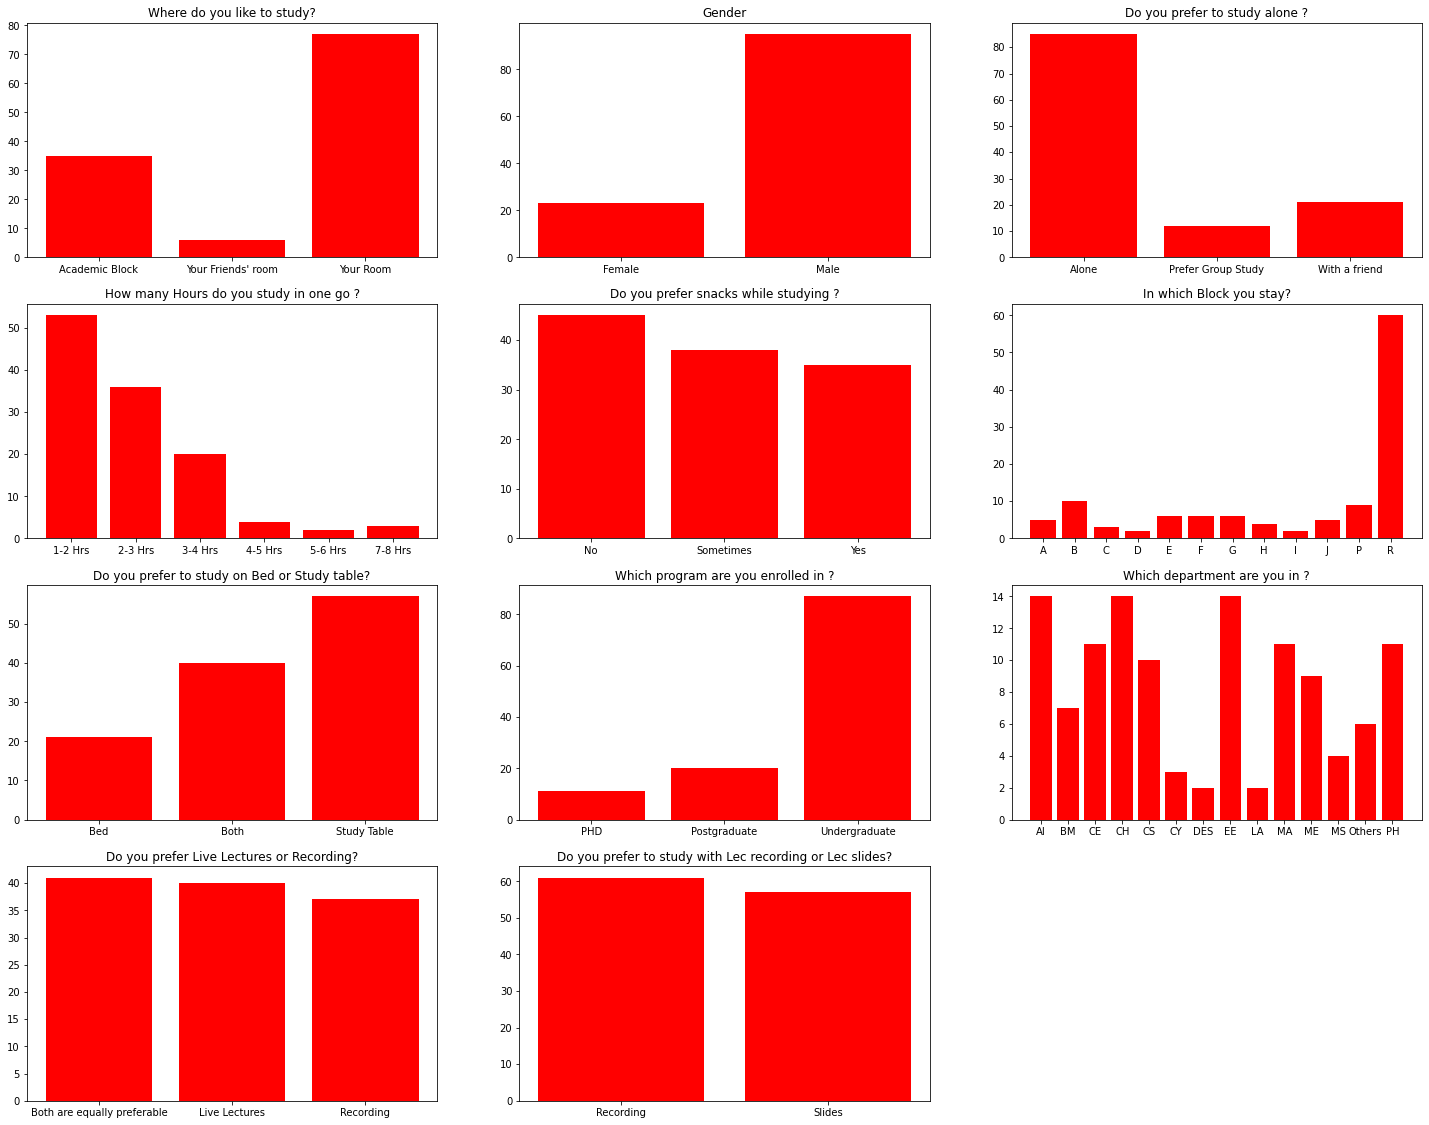
\includegraphics[scale=0.29]{output1.png}
    \caption{Visualizing the collected data}
    \label{fig:Visualized_data}
\end{figure}

\newpage
\section{Analysis and Conclusions}
\hspace{0.3in} After the pre-processing of the data, we had the data of 118 students from the survey, and we began to analyze the data. This involved the analysis of the one question that involved a numerical variable, that is: \\ \textbf{``How many hours do you study in one go?"}\\
The following results were obtained:
\begin{itemize}
    \item Mean $= 2.466$ hours
    \item Median $= 2.5$ hours
    \item Mode $= 2.5$ hours
\end{itemize}

\begin{figure}[h]
    \centering
    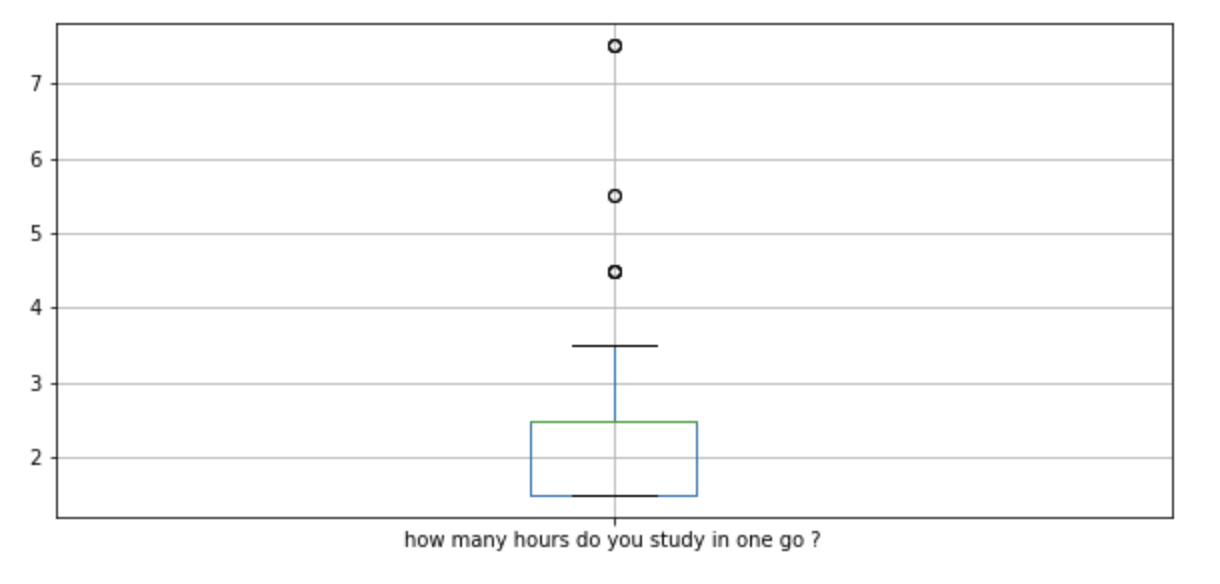
\includegraphics[scale=0.7]{output3.1.png}
    \caption{How many hours do you study in one go? (Box Plot)}
    \label{fig:study_hours}
\end{figure}

\begin{figure}
    \centering
    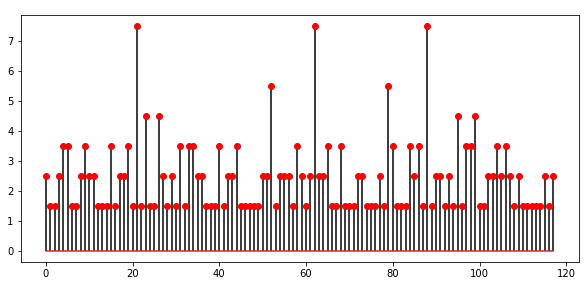
\includegraphics[scale=0.7]{output3.2.png}
    \caption{How many hours do you study in one go? (Stem Plot)}
    \label{fig:my_label}
\end{figure}

\hspace{0.3in} From the Box Plot: Figure \ref{fig:study_hours}, as well as the statistics, since the mean, median and mode are all approximately equal, we can say the data approximately follows a \underline{normal distribution}.\\
\vspace{5cm}

\hspace{0.3in} Doing some confidence testing for the mean of the data gives us the following:
\begin{itemize}
    \item A 95\% confidence interval is given by: (2.2388, 2.6934). \\The width of the interval is given by: 0.4546
    \item A 99\% confidence interval is given by: (2.1656, 2.7666). \\The width of the interval is given by: 0.6010
\end{itemize}

As expected, as we increase the confidence level, the width of the interval also increases. 
\newpage

A contingency table made from the data is as follows:
\begin{figure}[h]
    \centering
    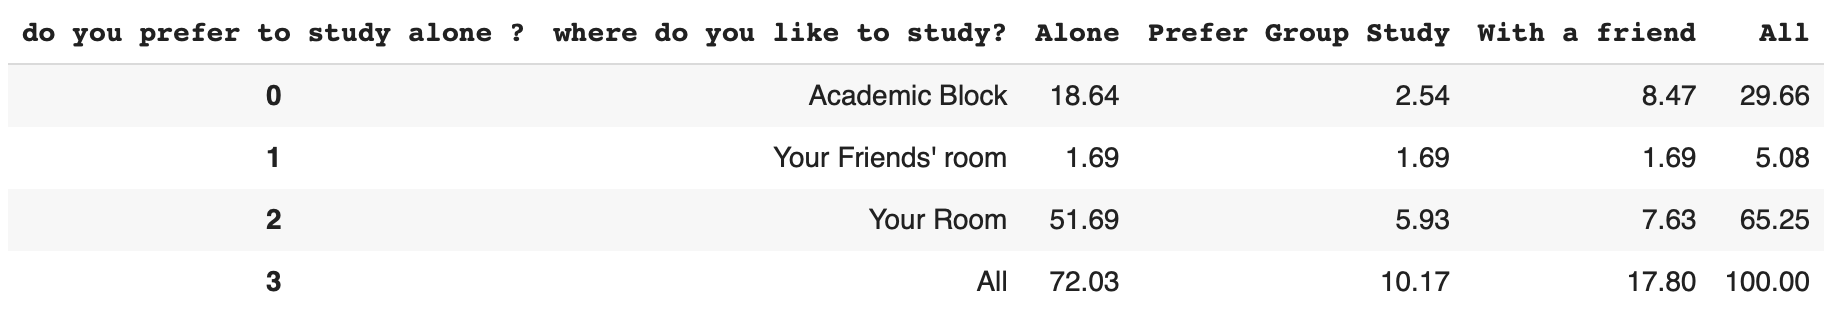
\includegraphics[scale=0.45]{output6.png}
    \caption{Contingency table for comparison of multiple categorical variables}
    \label{fig:contingency_table}
\end{figure}

After getting an idea of how the data stacks up, answers to some intriguing questions which involved the comparison of two questions were also given using segmented bar charts:

\begin{figure}[h]
    \centering
    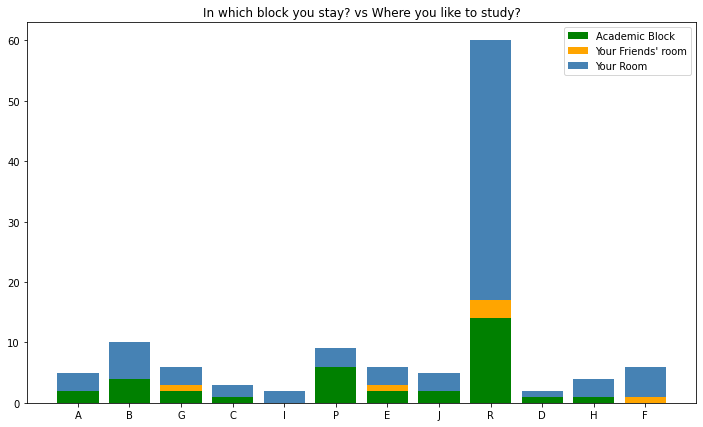
\includegraphics[scale=0.6]{output2.png}
    \caption{Residing Block vs Study room}
    \label{fig:stay_study}
\end{figure}
Based on the Segmented Bar Plot: Figure \ref{fig:stay_study}, the following conclusions can be made:
\begin{enumerate}
    \item A majority of students from the R block prefer to study in their rooms alone, whereas a majority of students from the P block (mainly involving Masters and Research students) prefer to go the academic blocks.
    \item Very few prefer to study in their friends' room. More or less, from every block, people want to study in their room itself.
\end{enumerate}
\newpage
\begin{figure}[h]
    \centering
    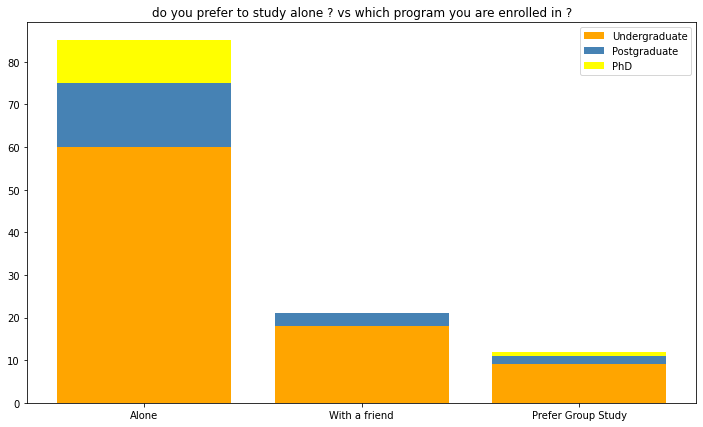
\includegraphics[scale=0.5]{output4.png}
    \caption{Preference towards studying alone vs Program}
    \label{fig:program_study}
\end{figure}
\hspace{0.3in} Based on the Segmented Bar Plot: Figure \ref{fig:program_study}, the following conclusion can be made:\\
Undergraduate students are open to studying alone, with a friend or even involving themselves in group studies. However, as we progress to Postgraduate and PhD students, they prefer studying alone in general.
\begin{figure}[h]
    \centering
    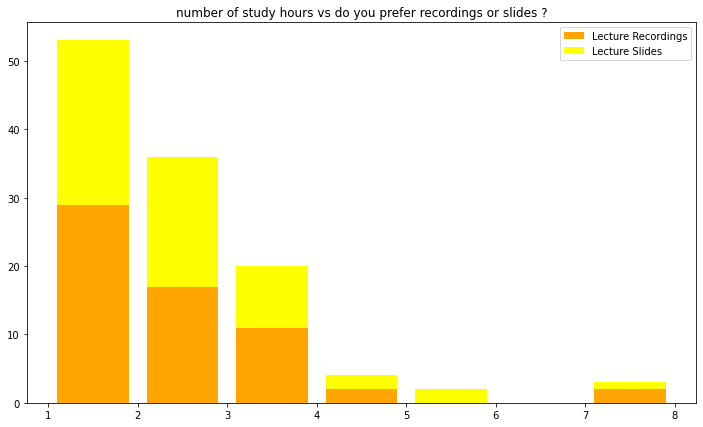
\includegraphics[scale=0.5]{output5.png}
    \caption{Hours studied vs Slides or Recordings}
    \label{fig:hour_slides}
\end{figure}

\hspace{0.3in} Based on the Segmented Bar Plot: Figure \ref{fig:hour_slides}, the following conclusion can be made:
More or less, equal number of people prefer lecture recordings and/or slides. However, most people who prefer recordings study for the minimum time at one go,
 and as this time tends to increase, people prefer to use slides to study.

\begin{figure}[h]
    \centering
    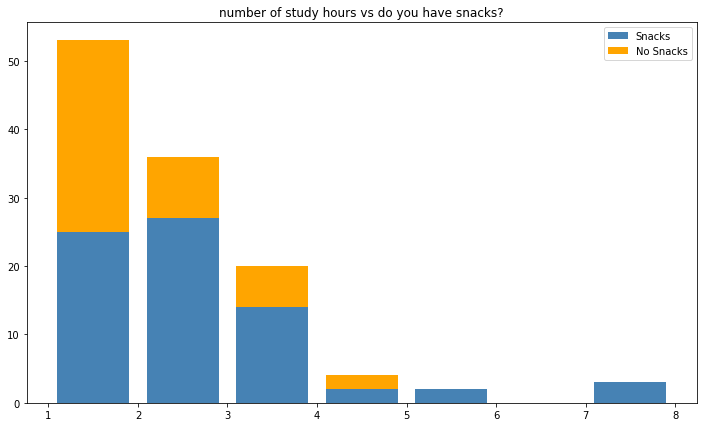
\includegraphics[scale=0.5]{snackstudytime.png}
    \caption{Study Hours vs Snacks Consumptions}
    \label{fig:hour_snack}
\end{figure}
\hspace{0.3in} Based on the Segmented Bar Plot: Figure \ref{fig:hour_snack}, the following conclusion can be made:\\
A larger proportion of people studying for longer hours prefer having snacks with them as compared to people studying just for $1-2$ hours 

\section {Hypothesis Testing:}
\subsection{Case-1: Comparing the study hours for Undergraduates and Postgraduates}
We compare study hours of Undergraduates and Postgraduates. We assume our null hypothesis to be that undergraduates study for longer duration than postgraduates. Let $\alpha = 0.05$\\

Let $\bar{x_1}$ = Sample Mean of study of Undergraduates \\
Let $\bar{x_2}$ = Sample Mean of study of Postgraduates \\
Let $S_1^2$ = Sample Variance of study of Undergraduates \\
Let $S_2^2$ = Sample Variance of study of Postgraduates \\ 

For Hypothesis Testing we make the following statements-
\begin{center}
    $ H_0 : \mu_1 - \mu_2 \geq 0$ and $H_a : \mu_1 - \mu_2 < 0$  \\
\end{center}

 We will now select a random sample of 18 entries  for the Undergraduates and 18 entries for the Postgraduates from our data. Based on the sample selected, we have the following information-
\begin{align}
    \bar{x_1} &= 2.50 \text{ hours}\\ 
    \bar{x_2} &= 2.37 \text{ hours} \\ 
    S_1^2 &= 1.219\\
    S_2^2 &= 1.335\\
    n_1 &= 81 \\
    n_2 &= 37\\
\end{align}
    
Since $\cfrac{S_1^2}{S_2^2} = 1.095 < 4$, we can assume the population variances would be equal. Thus, we can say: \par 
The degrees of freedom, $df = n_1 + n_2 -2 = 116$

 The pooled variance will be:
 \begin{align}
     S_p^2 &= \cfrac{(n_1-1)S_1^2 + (n_2-1)S_2^2}{n_1+n_2-2} = 1.255
 \end{align}
      
     

The test statistic is then given by:
 \begin{align}
      t &= \cfrac{\bar{x_1} - \bar{x_2} - 0}{s_p\sqrt{\cfrac{1}{n_1} + \cfrac{1}{n_2}}} = 0.584
 \end{align}
    
 \par
 Using the rejection region approach, we reject $H_0$ if $t \leq -t_{0.05, 116}$, where $t_{0.05,116} = -1.658$.\\ 
 Because the observed value of $t=0.584$ is less than $1.658$, we have enough statistical evidence to reject the null hypothesis, and thus, we can say, the postgraduates study more in one go than the undergraduates on average.

\subsection{Case-2: Comparing the study hours of people who study alone and who study in groups.}
We compare study hours of people studying alone and in groups. We assume our null hypothesis that people studying alone study for longer time.\\

Let $\bar{x_1}$ = Sample Mean of study hours of people studying alone \\
Let $\bar{x_2}$ = Sample Mean of study hours of people studying in groups \\
Let $S_1^2$ = Sample Variance of study hours of people studying alone \\
Let $S_2^2$ = Sample Variance of study hours of people studying in groups \\ 

For Hypothesis Testing we make the following statements-
\begin{center}
    $ H_0 : \mu_1 - \mu_2 \geq 0$ and $H_a : \mu_1 - \mu_2 < 0$  \\
\end{center}

\begin{align}
    \bar{x_1} &= 2.488 \text{ hours}\\ 
    \bar{x_2} &= 2.409 \text{ hours} \\ 
    S^2_1 &= 0.535\\
    S^2_2 &= 0.647\\
    n_1 &= 85\\
    n_2 &= 33
\end{align}
    
Since $\cfrac{S_1^2}{S_2^2} = 1.209 < 4$, we can assume the population variances would be equal. Thus, we can say: \par The degrees of freedom, $df = n_1 + n_2 -2 = 116$

 The pooled variance will be:
 \begin{align}
     S_p^2 &= \cfrac{(n_1-1)S_1^2 + (n_2-1)S_2^2}{n_1+n_2-2} = 0.5658
 \end{align}
      
     

The test statistic is then given by:
 \begin{align}
      t &= \cfrac{\bar{x_1} - \bar{x_2} - 0}{s_p\sqrt{\cfrac{1}{n_1} + \cfrac{1}{n_2}}} = 0.512
 \end{align}

 \par
 Using the rejection region approach, we reject $H_0$ if $t \leq -t_{0.05, 116}$, where $t_{0.05,116} = -1.658$.\\ 
 Because the observed value of $t=0.512$ is less than $1.658$, we have enough statistical evidence to reject the null hypothesis, and thus, we can say, those who study in groups study more on average in one go than those who study alone.
 
\subsection{Case-3: Comparing the study hours of people who study while eating snacks and who study without eating snacks.}
We compare study hours of people studying while eating snacks and those who prefer not to! We assume our null hypothesis that people studying while eating snacks study for longer time.\\

Let $\bar{x_1}$ = Sample Mean of study hours of people studying while eating snacks \\
Let $\bar{x_2}$ = Sample Mean of study hours of people studying without eating snacks \\
Let $S_1^2$ = Sample Variance of study hours of people studying while eating snacks \\
Let $S_2^2$ = Sample Variance of study hours of people studying without eating snacks \\ 



For Hypothesis Testing we make the following statements-
\begin{center}
    $ H_0 : \mu_1 - \mu_2 \geq 0$ and $H_a : \mu_1 - \mu_2 < 0$  \\
\end{center}

\begin{align}
    \bar{x_1} &= 2.671 \text{ hours}\\ 
    \bar{x_2} &= 2.379 \text{ hours} \\ 
    S^2_1 &= 0.91\\
    S^2_2 &= 0.4\\
    n_1 &= 35\\
    n_2 &= 83
\end{align}

Since $\frac{S_1^2}{S_2^2} = 2.275 < 4$, we can assume the population variances would be equal. Thus, we can say: \par The degrees of freedom, $df = n_1 + n_2 -2 = 116$

 The pooled variance will be:
 \begin{align}
     S_p^2 &= \cfrac{(n_1-1)S_1^2 + (n_2-1)S_2^2}{n_1+n_2-2} = 0.55
 \end{align}
      

The test statistic is then given by:
 \begin{align}
      t &= \cfrac{\bar{x_1} - \bar{x_2} - 0}{s_p\sqrt{\cfrac{1}{n_1} + \cfrac{1}{n_2}}} = 1.9685
 \end{align}

 \par
 Using the rejection region approach, we reject $H_0$ if $t \leq -t_{0.05, 116}$, where $t_{0.05,116} = -1.658$.\\ 
 Because the observed value of $t=1.9685$ is greater than $1.658$, we fail to reject the null hypothesis, and thus, do not have enough evidence to say that those who eat snacks while studying study for longer at one go than those who do not.


\subsection{Case-4: Comparing the study hours of people who study from Lecture Slides and those who study from Lecture Recordings.}

We compare study hours of people studying from lecture slides and those who study from lecture recordings! We assume our null hypothesis that people studying from slides study for longer time than those who study from lecture recordings.\\

Let $\bar{x_1}$ = Sample Mean of study hours of people studying from slides \\
Let $\bar{x_2}$ = Sample Mean of study hours of people studying from recordings \\
Let $S_1^2$ = Sample Variance of study hours of people studying from slides \\
Let $S_2^2$ = Sample Variance of study hours of people studying from recordings \\ 

For Hypothesis Testing we make the following statements-
\begin{center}
    $ H_0 : \mu_1 - \mu_2 \geq 0$ and $H_a : \mu_1 - \mu_2 < 0$  \\
\end{center}

\begin{align}
    \bar{x_1} &= 2.5 \text{ hours}\\ 
    \bar{x_2} &= 2.43 \text{ hours} \\ 
    S^2_1 &= 0.5\\
    S^2_2 &= 0.629\\
    n_1 &= 57\\
    n_2 &= 61
\end{align}

Since $\frac{S_1^2}{S_2^2} = 1.258 < 4$, we can assume the population variances would be equal. Thus, we can say: \par The degrees of freedom, $df = n_1 + n_2 -2 = 116$

 The pooled variance will be:
 \begin{align}
     S_p^2 &= \cfrac{(n_1-1)S_1^2 + (n_2-1)S_2^2}{n_1+n_2-2} = 0.5764
 \end{align}
      

The test statistic is then given by:
 \begin{align}
      t &= \cfrac{\bar{x_1} - \bar{x_2} - 0}{s_p\sqrt{\cfrac{1}{n_1} + \cfrac{1}{n_2}}} = 0.5
 \end{align}

 \par
 Using the rejection region approach, we reject $H_0$ if $t \leq -t_{0.05, 116}$, where $t_{0.05,116} = -1.658$.\\ 
 Because the observed value of $t=0.5$ is lesser than $1.658$,we have enough statistical evidence to reject the null hypothesis, and thus, we can say, those who study from recordings study more on average in one go than those who study from slides.

\newpage
\section {Contributions:}

\begin{itemize}
    \item \textbf{Varunaditya Singhal}
    \begin{itemize}
        \item The idea of the  Project.
        \item Making Questions along with the google form.
        \item Data collection for the project
        \item pre-processing of data.
        \item Hypothesis testing of 3 scenarios along with the code for same.
        \item Making report in \LaTeX
    \end{itemize}
    
    \item \textbf{Prakhar Patni}
    \begin{itemize}
    \item Ideation for the project
        \item Data collection for the project
        \item Ideation for Hypothesis testing
        \item Making report in \LaTeX
    \end{itemize}
    \item \textbf{Tanmay Goyal}
    \begin{itemize}
        \item Ideation for the project
        \item Helping with the pre-processing of data
        \item \LaTeX \hspace{0.03cm} report and drawing
        conclusions
        \item Assisted with Hypothesis Testing ideation, and code for the same.
        \item Collab Notebook organisation and clean-up
    \end{itemize}
    \item \textbf{K N Vardhan}
    \begin{itemize}
        \item Ideation for the project
        \item Analyzing the Uni-variate Numerical dataset and drawing conclusions
        \item Visualizing few of the categorical datasets with segmented bar charts
        \item Assisted in hypothesis testings
        \item Making presentation slides
    \end{itemize}
    \item \textbf{Tanay Yadav}
    \begin{itemize}
        \item Ideation for the project
        \item Pre-processing the data using Pandas in Python
        \item Visualizing few of the categorical datasets with segmented bar charts
        \item Making report in \LaTeX
    \end{itemize}
    \item \textbf{Sujal}
     \begin{itemize}
        \item Ideation for the project
        \item Made presentation
        
    \end{itemize}
\end{itemize}


\end{document}
